\chapter{Columnar Compression}
\label{columnar-compression}

Compressing data stored in columns and query processing directly on compressed data have been extensively studied in the context of column-oriented \gls{rdbms}s. These techniques are directly relevant to our work. However, not all columnar compression techniques can be directly applied to the data-structures that we introduced in Chapter~\ref{c:columnar-storage}. Recall our Desideratum~\ref{des:compression} that in the context of in-memory GDBMSs, we are interested in compression schemes that either avoid decompression at all or decompress arbitrary single elements in a compressed block in constant time. For example, schemes such as run-length encoding are not suitable for in-memory GDBMSs because it is not possible to decompose the value of an arbitrary element in constant time. We begin in Section~\ref{sec:col-existing} by reviewing a number of existing compression techniques that satisfy this constraint and where they can be applied in GDBMSs. In Section~\ref{sec:storage-optimizations} we discuss opportunities where we can compress our adjacency lists, i.e., the storage of (edge ID, neighbour ID) pairs, given our new ID schemes. Finally, in Section~\ref{sec:null}, we discuss the shortcomings of directly applying existing null compression schemes from columnar RDBMSs to compress null values or empty lists in GDBMSs and propose a new \emph{prefixSum-based null compression} scheme that is suitable for GDBMSs.

\section{Directly Applicable Compression Techniques}
\label{sec:col-existing}

%We designed our columnar data structures for in-memory \gls{gdbms}. For these data structures, the focus with compression is not on achieving high compression ratios but to optimize for high decompression rates or to avoid decompression of data at all. There has been much research that studies compression techniques from the point of avoiding eager decompression of compressed data \cite{westmann-comp, dat-comp}. \cite{abadi-col-comp} abstracts out the high-level properties of a compression algorithm and use this information in query executor to operate directly on compressed data whenever possible. Our's is an identical requirement in the sense that operating directly on compressed data can avoid CPU overhead and increases the read throughput while reading from adjacency lists and property stores.
%
%The design of vertex and edge property columns as described in sections \ref{sec:vertex-property-columns} and \ref{sec:edge-property-columns}, allows for random access of property values based on the positional offset in a column. Random lookups in a column can be performed intuitively once we decompress the entire column or a part of it. However, this involves the additional cost of decompressing elements that are not required to be read, thereby wasting CPU cycles. We can avoid this cost by randomly acessing elements from the compressed column, which is a step ahead of operating directly on the compressed data. 
Random access to a compressed column is possible only if the elements of a column are encoded in \emph{fixed-length codes}, i.e. using a fixed number of bits, instead of variable-length codes. Several existing schemes, such as dictionary encoding, leading 0 suppression, bit vectors, and frame of reference produces fixed length codes. We review dictionary encoding and leading 0 suppression below, which we have integrated in our implementation. We refer the readers to references~\cite{abadi-col-comp, goldstein:for, lemire:integer} for details of other schemes.
We next review several of existing techniques that produce fixed length codes.

%The only columnar compression techniques that keep the data in fixed-width bits are \emph{dictionary encoding} and \emph{bit-vector encoding}. Whereas, related techniques, \emph{Prefix Supression} and \emph{Frame of Reference (FOR)}, can be adopted to encode elements in fixed-bitwidth to make them appropriate for our case. For each of these techniques, we give a brief description of the technique and state its characteristics that makes it suitable for our use-case. We also give a high-level implementation of how a technique is used in our system.
\noindent \textbf{Dictionary encoding:} The dictionary encoding is perhaps the most common encoding scheme to be used in \gls{rdbms}s~\cite{abadi-col-comp, boncz-comp}. At a high-level, this scheme maps a domain of values into more compact and shorter representations using a variety of schemes \cite{boncz-comp, dat-comp, abadi-col-comp}. Some of these schemes produce variable-length codes, such as Huffmann encoding, and others use fixed-length codes, such as the one described in reference\cite{abadi-col-comp}. These techniques are often used to encode \texttt{STRING}s into 64-bit integer values or any categorial property into a small number of fixed-length bits. Different schemes can further pack these bits into bytes. In our implementation, we use dictionary encoding to map any categorial property $p$ that takes on $z$ different many values to  $\lceil log_2(z)/8 \rceil$ bytes (so we pad $log_2(z)$ bits with 0s to have a fixed number of bytes).
	
%\noindent \textbf{Bit-vector encoding:} The bit-vector encoding scheme is used to encode columns with small number of unique elements. It encodes the column by having $n$ bit-strings, one for each unique element. A bit-string associated to the value has the bit set at positions where that value appears in the column. Accessing a random location $i$ in a column compressed by bit-vector involves inspecting the $i$th position of each bit-string till a set bit is found. Inspecting \emph{all} the bit-strings adds to the overhead which increases with the number of unique values in the column. Hence, encode a column using bit vectors only when the unique values are less than 50.
	
\noindent  \textbf{Leading 0 Suppression:} Given a block of data, this scheme omits storing leading zero bits or in each value in the block \cite{beckmann:sparse}. Each value is, hence, encoded in a variable number of bits along with the count of bits used for storing the value. For an integer value 12, the number of bits in which it can be stored is 4, instead of default 32. There are both variable-length and fixed-length variants of this scheme. We adopt a fixed length version where for storing labels and positional offsets in both edge and vertex IDs (though it is trivial to apply to vertex and edge properties as well). Specifically, if there $max_v$ many vertices of a particular label, we store the positional offsets in $\lceil log_2(max_v)/8\rceil$ many bytes instead of 8 bytes. Similarly, if the maximum size of a property page of an edge label is $k$, for all for all the associated edges, we use $\lceil log_2(k)/8\rceil$ many bytes for the page-level positional offset of the edge ID. Often the forward adjacency lists of many edge labels are quite small (even the maximum length one), and we store the positional offsets with a few bytes, instead of 4 bytes. Similarly if there are $max_{\ell}$ many different labels, we store labels as in $\lceil log_2(max_{\ell})/8\rceil$ many bytes. That said, during query processing and accessing properties, the  labels, positional offsets of vertices, and positional offset of edges are stored as 4, 8 and 4 bytes, respectively.

%\begin{enumerate}
%		\item To make this encoding byte-aligned and easy to decompress, we store the values in variable bytes instead of in variable number of bits. Hence, an integer value can be encoded with either 1, 2, 3 or 4 bytes, with two extra bits needed to store the number of bytes. 
%		\item We do not encode each element of the column separately in variable-bitwidth. Instead, the element is encoded in the number of bytes that is sufficient to encode the largest element in a column or a block in column. The number of bytes for encoding an element is, hence, given by $\lceil log_2(max_v+1)/8\rceil$, where $max_v$ is the maximum element in the column or block. The resultant column now has fixed-bitwidth elements and does not need to store an extra 2 bits for the number of bytes used.
%	\end{enumerate}

%\noindent  \textbf{Frame Of Reference(FOR): }This technique is similar to the previous, instead each element $e$ is stored as NULL supressed $e-b$, $b$ is called the \emph{base value} of the column or block. Generally, for an integer column, its smallest element is take as the base value. FOR is effective when the elements of column are clustered.
	
\section{Compressed Storage of Edge and Vertex ID Pairs in Adjacency Lists}
\label{sec:storage-optimizations}

We next discuss how to compress the edge ID and vertex ID pairs in the adjacency lists. Our new ID schemes from Sections \ref{sec:vertex-property-columns} and \ref{sec:edge-property-columns} decompose the IDs into multiple small components, which enables us to factor out most of these components, when the data depicts some structure. 

Recall that the ID of an edge $e$ in our new edge ID scheme contains 4 components: (i) edge label; (ii) source vertex ID; (iii) destination vertex ID; and (iv) positional offset of the properties of $e$ in property pages. Recall also that then ID of a vertex $v$ contains 2 components: (i) vertex label; and (ii) (label-level) positional offset. First, both the source and the destination vertex IDs inside the edge ID of (edge ID, neighbor ID) pairs can be omitted. This is because the source (destination) vertex ID is implied by the offset of the pair in the forward (backward) adjacency list and the destination (source) vertex ID is the neighbor ID, which is already stored in the pair. Second, we do not have to store the labels of the edges as in our storage of the adjacency lists because recall that we store a different \gls{csr}-like structure for each edge label. Therefore the only parts that need to be stored are positional offsets for edge IDs, and vertex label and positional offsets of neighbor IDs. We next discuss further cases when the structure and multiplicities of edges allows us to factor some of these components out: 
%Finally, the positional offset can be stored cheaply as often they are not more than 1 or 2 bytes hence. This follows from the fact that the number of edges in most of the adjacency list is relatively small (by the power-law) and so are the number of elements in each page. 

%To sum up, each entry in the adjacency list stores a small (1-2 byte) positional offset and the neighbour vertex ID which itself comprises of vertex label and local positional offset. We now present some common scenarios that allow for even further compaction by choosing to omit to store certain components:

\begin{figure}
	\centering
	\begin{tikzpicture}[node distance=3cm]
	\node (edge) [io] {edge $e$};
	\node (dec1) [decision, below of=edge] {has 1 neighbour label?};
	\node (p1) [process, below of=dec1] {Do not store neighbour vertex label};
	\node (p2) [process, right of=dec1, xshift=1cm, yshift=-2.8cm] {store neighbour vertex label};
	\draw [arrow] (edge) -- (dec1);
	\draw [arrow] (dec1) -- node[anchor=east] {yes} (p1);
	\draw [arrow] (dec1) -| node[anchor=south] {no} (p2);
	\end{tikzpicture}
	\captionsetup{justification=centering}
	\caption{Decision tree to store neighbour vertex's label in the Adjacency lists.}
	\label{fig:dec1}
\end{figure}

\begin{itemize}
	\item \textbf{Edge label determines a single neighbour vertex label.} In this very frequent case, an edge label is between pairs of nodes when the sources or destinations (or both) can have a single label. For instance, in our example graph, \texttt{FOLLOWS} edges are between vertices having the label \texttt{PERSON}. In this case, we can factor out the vertex label component of neighbor ID.
		
	\item \textbf{Edges do not have properties:} This is also a frequently appearing case. That is the edges with a particular label do not have any structured or unstructured properties. In this case, notice that the edges do not need to be identifiable at all as the system will never access properties of these edges. Therefore, what distinguishes two edges are their neighbor IDs and edges with the same IDs are simply replicas of each other and are stored twice. Therefore, we can omit storing the positional offsets of edge IDs.
	
	\item \textbf{Single cardinality edges:} Recall from Section~\ref{sec:single-cardinality-cols} that the properties for single cardinality edges can be stored in vertex property columns. So by using the source or destination vertex IDs, we can directly read properties. Therefore, we can omit storing any positional offsets. 
		
\end{itemize}

\begin{figure}
	\centering
	\begin{tikzpicture}[node distance=3cm]
	\node (edge) [io] {edge $e$};
	\node (dec1) [decision, below of=edge] {single cardinality?};
	\node (p1) [process, below of=dec1] {Do not store positional offsets};
	\node (dec2) [decision, right of=dec1, xshift=1.2cm] {has properties?};
	\node (p2) [process, right of=dec2, xshift=-0.5cm, yshift=-3cm] {store positional offsets};
	\draw [arrow] (edge) -- (dec1);
	\draw [arrow] (dec1) -- node[anchor=east] {yes} (p1);
	\draw [arrow] (dec1) -- node[anchor=south] {no} (dec2);
	\draw [arrow] (dec2) |- node[anchor=south, xshift=-1cm] {no} (p1);
	\draw [arrow] (dec2) -| node[anchor=south] {yes} (p2);
	\end{tikzpicture}
	\captionsetup{justification=centering}
	\caption{Decision tree to store edge's positional offset in the Adjacency lists.}
	\label{fig:dec2}
\end{figure}

All of the above cases arise frequently in real world graph data. For example, in the \gls{ldbc} dataset~\ref{fig:ldbc-schema}, 10  out of 15 many edge labels determine a single source and destination neighbour label, 10 many do not have any properties, 8 many have single cardinality edges. In all, 10 many of them are not required to store any neighbour vertex's labels and positional offset. This implies that we only store neighbour vertex's positional offset for such edges in the adjacency lists, which can be stored with as few as 4 bytes.

Figures~\ref{fig:dec1} and ~\ref{fig:dec2} summarizes these cases in a decision tree that instruct when to omit storing certain components.

% **** Let's not call NULL compression but "trailing 0 omission" and I think let's not talk about factoring things out 
%Using the new identification scheme and further applying the above-mentioned optimizations, the adjacent edges and neighbour vertices in adjacency lists by as less as a single piece of information. We can still further reduce the memory footprint of adjacency lists by applying compression on components of the edge that has to be stored after removing unnecessary ones. We use \emph{fixed-bitwidth NULL compression}, which we describe in Section~\ref{sec:col-existing}, to compress the components of edge in the adjacency lists. Using this technique, a particular component of each edge in an adjacency list is encoded as fixed-width elements by removing a common number of leading zero bytes (that will be determimined by the maximum element) from each of them. For example, if an adjacency list has edge $[e1, e2, e3, e4, e5]$ with the neighbour vertex labels $[1, 2, 1, 1, 2]$, then the neighbour vertex label is encoded in 1 byte in the adjacency list, instead of usual 4-byte INT. Similarly, if the same set of edges have neighbour's local positional offsets $[1000, 2000, 3000, 2, 1]$, then each offset is stored in 2 bytes in the adjacency list.

%We show the decrease in memory footprint of the adjacency lists, with each optimization, over the LDB SnB dataset, with more than 1 billion edges, in Chapter~\ref{c:evaluation}. Our evaluations reveal that the new scheme with opportunities to perform immense compaction and compression can reduce the size of adjacency lists by upto 94x, storing barely over 6 bytes of data per indexed edge in the system.

\section{NULL Compression}
\label{sec:null}

Edge and vertex properties can often be quite sparse in real-world graph structured data. Similarly in many adjacency lists, due to the power-law nature of the degree distributions, a significant fraction of vertices can have empty forward or backward adjacency lists. Both the property sparsity and empty lists can be seen as different columnar structures containing null values, which can be compressed.

%Owing to the nature of property graph data, one can expect a large number of \texttt{NULL} values, even in the columns for structured properties. Hence, the compression scheme is required to avoid storing \texttt{NULL} values in the columns, in order to reduce memory footprint of sparse columns. Even with storing only the not-\texttt{NULL} elements in a column, it is desirable to access an element from the column randomly and in constant time without decompressing. 

A general null compression technique is to treat the \texttt{NULL}s in the column as another potential value in the domain of column's datatype which could then be compressed by any of the columnar compression schemes. For example, a column that is very sparse ($>95\%$ \texttt{NULL} values) can be effectively encoded using run-length encoding. This is not directly applicable in GDBMSs as it does not allow accessing an arbitrary location in a column and finding the value (or null if the value does not exist).

Abadi in reference \cite{abadi-sparse-col} has described three specific \texttt{NULL} compression techniques. All of these techniques list all non-\texttt{NULL} elements consecutively in a block of data. Then to indicate the positions of these non-\texttt{NULL} elements, they use different techniques. The simplest is to list along with each value the position. Borrowing the terminology from reference \cite{abadi-sparse-col}, this technique is designed for sparse columns, i.e., whose significant fraction of values, say $> 90\%$ are \texttt{NULL}. A more compact way, designed for columns that have low sparsity, is to list in a separate array the beginning and end indices of consecutive non-\texttt{NULL} values. The third technique, designed for columns with intermediate sparsity, is based on using bit-string to indicate if each location is \texttt{NULL} or not.  This is quite compact and requires only 1 bit extra storage per each cell in the block. Figure \ref{fig:null1} shows an example column and its null compressed version using the bit-string scheme. 

\begin{figure}
	\hfill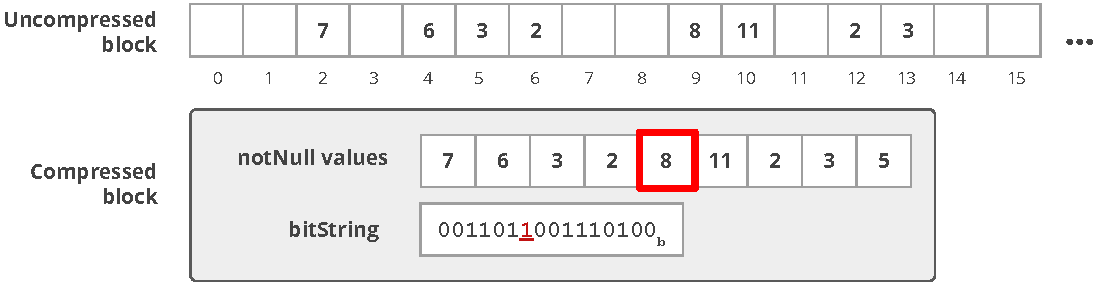
\includegraphics[scale=0.70]{img/null1}\hspace*{\fill}
	\captionsetup{justification=centering}
	\caption{\texttt{NULL} compression using bit-Strings.}
	\label{fig:null1}
\end{figure}

%The column is divided into block, where each compressed block holds 2 pieces of information: 1) a \textbf{non-\texttt{NULL}s array} that holds the non \texttt{NULL} values of the uncompressed block, and 2) a \textbf{bit-string} having a bit for each element in block, with 1's for non NULL elements. The storage overhead of the compressed block is only that of the bit-string which is 1 bit per element in the uncompressed block or 0.5 bit per non NULL element of the block that is 50\% occupied. Based on the sparsity, bit-string can be replaced by a list of offsets of non \texttt{NULL} elements in block for very sparse data, or list or ranges of non \texttt{NULL} elements for very dense data.

However, these techniques are not directly suitable for GDBMSs as they do not satisfy our Desideratum~\ref{des:compression}. In the bit-string method, we can in constant time learn whether or not if the value at a position $i$ is \texttt{NULL} or not (e.g., $i$ would be the positional offset of a vertex in a column storing a vertex property). However, if the value is not \texttt{NULL}, the system needs to iterate over the bits until location $i$ and count the number of $1$'s to find out the location of the value. For instance, in Figure~\ref{fig:null1}, accessing the element at index 9 of uncompressed block involves counting the number of 1's till before index 9 in the bit-string, which is 4. Thus, the value is then read from index 4 of the non-\texttt{NULL} values array. 

%Even though it is possible to operate on compressed column, the proposed scheme do not cater to our requirement of constant time random access. Reading from the compressed block involves iterating over the bit-string to calculate the location of the element in the non-\texttt{NULL}s array.

%\section{PrefixSum-based NULL Compression}
%\label{sec:prefixbased}

\begin{figure}
	\hfill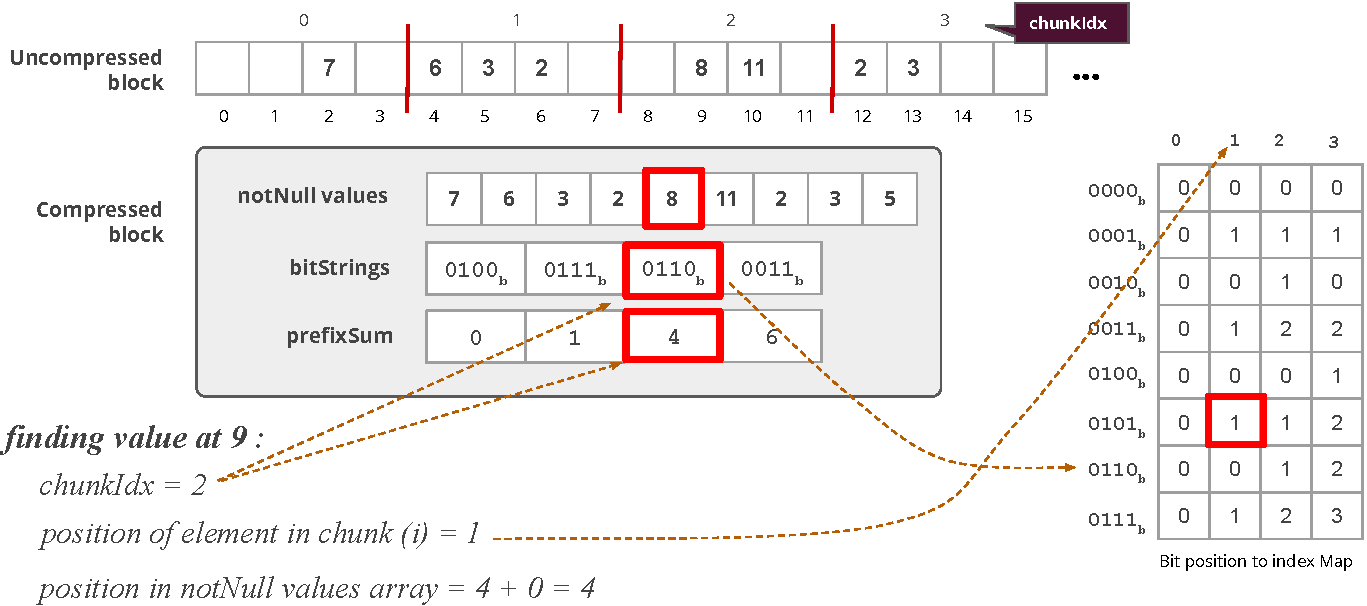
\includegraphics[scale=0.70]{img/null2}\hspace*{\fill}
	\captionsetup{justification=centering}
	\caption{PrefixSum-based \texttt{NULL} compression scheme. Chunk Size (n) = 4}
	\label{fig:null2}
\end{figure}

We next present a modification to the bit-string-based compression scheme to satisfy our requirement of constant time access to arbitrary elements. In addition to the array of non-\texttt{NULL} values and the bit-string, we store a prefixSum for each $c$ (16 by default) elements in a block of the column, i.e., we divide the block into chunks of size $c$. While the bit-strings indicate positions in the block with non \texttt{NULL} elements, the prefixSum holds the number of non \texttt{NULL} elements in the uncompressed block before a particular chunk. We also maintain a pre-populated static 2D map in the memory having size $(2^c, c)$. We call this \emph{bit-position-to-index map}. Let $b$ and $p$ respectively be the bit-string of length $c$ and prefixSum of a chunk $j$. Given $b$ and the position $i$ in the bit-string, the map returns the number of 1's in $b$ until position $i$. The map  allows us to avoid iterating over the bit-string to count the number of 1s and perform this count with a single lookup. Then, by adding the value returned from the map to $p$, we get the exact location of the value of location $i$ in $j$ (so the location of $j*c + i$ in the entire block). In total, after checking that the value is non-\texttt{NULL}, which needs to be done in any bit-string based scheme, we perform 1 lookup of prefix, 1 look up in the map, and 1 arithmetic, before the final look up of the actual value in the non-\texttt{NULL} values array.

%Therefore with 1 map lookup, 1 look1 arithmetic andFigure~\ref{fig:null2} depicts this prefix-sum-based null compression scheme. 

%We can directly to get the index of the element, at $i$ in the chunk, in the non-\texttt{NULL}s array. The index value returned by the map is relative to that chunk. This value, when added to $p$, gives the absolute index of the element, at $i$ in the chunk, in the non-\texttt{NULL} values array of the element.

% The prefixes at location $j$ indicates the total number of non-null values among the first $c*i$ locations in the column.  

%the solution to overcome the problem of constant time random reads in the existing solutions for compressing \texttt{NULL}s in sparse columns. The high-level idea is to do away with iteration over the bit-string while accessing the particular element in the compressed column.

%Figure~\ref{fig:null2} depicts compression of a sparse column using our scheme, which we call \emph{prefixSum-based null compression}. It divides a block into chunks of fixed size $n$. A compressed block contains 3 pieces of information: 1) a non-\texttt{NULL}s array, 2) an array of bit-strings and, 3) an array of prefixSums. We store one bit-string of length $n$ and a prefixSum per chuck. Whereas the bit-string indicates positions in the chunk with non \texttt{NULL} elements, the prefixSum holds the number of non \texttt{NULL} elements in the uncompressed block before the current block. 

Figure~\ref{fig:null2} depicts compression of a sparse column using our modified scheme. As an example, suppose we need to find the element at index 9 of the uncompressed block. Given $c=4$, this element will appear in the 2nd chunk, say $c_2$, of the compressed block. The position $i$ of index 9 in $c_2$ is 1. Also, $c_2$'s bit-string and prefixSum are $\texttt{0110}_b$ and 4 respectively. The entry for ($\texttt{0110}_b$, 1) in the bit-position-to-index map is 0. Thus, the index of element at 9 in non-\texttt{NULL} values array is $4+0 = 4$.

The choice of the value of $c$ affects how big the bit index to position map is. For $c = 16$, the size of the map is 1MB. The overhead of bit-string and prefixSum can also be optimized. Since the bit-string takes a bit for each element in an uncompressed block, the overhead depends on the size and number of prefixSums we have for an uncompressed block. By default we set $c$ to 16 and maintain blocks of size $N=2^c$ (so about 64K cells) and store our prefixSums as 16-bit unsigned integers. This ensures that the prefixes we keep increase the overhead from 1 to only 2 bits per element in the compressed block. If the size of prefixSum is $w$ and $c=16$, the overhead from prefixSums per element will be $w/16$ bytes. $w$ itself depends on the number of elements $N$ in the uncompressed block. For $N=2^{16}=64K$, $w=16$ and hence, the overhead of prefixSum is 1-bit per each cell in the block.

In our implementation, we use the prefix-sum based \texttt{NULL} compression schemes to compress vertex and edge properties (so vertex property columns and single-directional property pages) as well as empty lists in adjacency lists.  
%Our NULL compression scheme can be used orthogonally with any of the applicable columnar compression techniques that we discussed in section~\ref{sec:col-existing}. 
%We evaluate the effectiveness of our scheme in Chapter~\ref{c:evaluation} in effect to the storage savings by avoiding \texttt{NULL}s and the performance of queries when operating on \texttt{NULL} compressed columns.
















